% Created 2015-01-18 dom 10:46
\documentclass[xcolor={usenames,svgnames,dvipsnames}]{beamer}
\usepackage[utf8]{inputenc}
\usepackage[T1]{fontenc}
\usepackage{fixltx2e}
\usepackage{graphicx}
\usepackage{longtable}
\usepackage{float}
\usepackage{wrapfig}
\usepackage{rotating}
\usepackage[normalem]{ulem}
\usepackage{amsmath}
\usepackage{textcomp}
\usepackage{marvosym}
\usepackage{wasysym}
\usepackage{amssymb}
\usepackage{hyperref}
\tolerance=1000
\usepackage{color}
\usepackage{listings}
\usepackage{mathpazo}
\usepackage{gensymb}
\usepackage{amsmath}
\bibliographystyle{plain}
\AtBeginSubsection[]{\begin{frame}[plain]\tableofcontents[currentsubsection,sectionstyle=show/shaded,subsectionstyle=show/shaded/hide]\end{frame}}
\AtBeginSection[]{\begin{frame}[plain]\tableofcontents[currentsection,hideallsubsections]\end{frame}}
\usepackage[emulate=units]{siunitx}
\sisetup{per=fraction, fraction=nice, decimalsymbol=comma}
\newunit{\wattpeak}{Wp}
\newunit{\watthour}{Wh}
\newunit{\amperehour}{Ah}
\hypersetup{colorlinks=true, linkcolor=Blue, urlcolor=Blue}
\setbeamercolor{alerted text}{fg=red!50!black} \setbeamerfont{alerted text}{series=\bfseries}
\usetheme[hideothersubsections]{Goettingen}
\usecolortheme{rose}
\usefonttheme{serif}
\author{Oscar Perpiñán Lamigueiro \\ \url{http://oscarperpinan.github.io}}
\date{}
\title{Energía Solar Fotovoltaica:\\Célula Solar}
\hypersetup{
  pdfkeywords={},
  pdfsubject={},
  pdfcreator={Emacs 24.4.1 (Org mode 8.2.7c)}}
\begin{document}

\maketitle

\section{Teoría de Semiconductores}
\label{sec-1}

\subsection{Modelo de bandas de energía}
\label{sec-1-1}

\begin{frame}[label=sec-1-1-1]{Átomos aislados vs. Átomos en Sólido}

\href{http://upload.wikimedia.org/wikipedia/commons/8/81/Metals_and_insulators,_quantum_difference_from_band_structure.ogv}{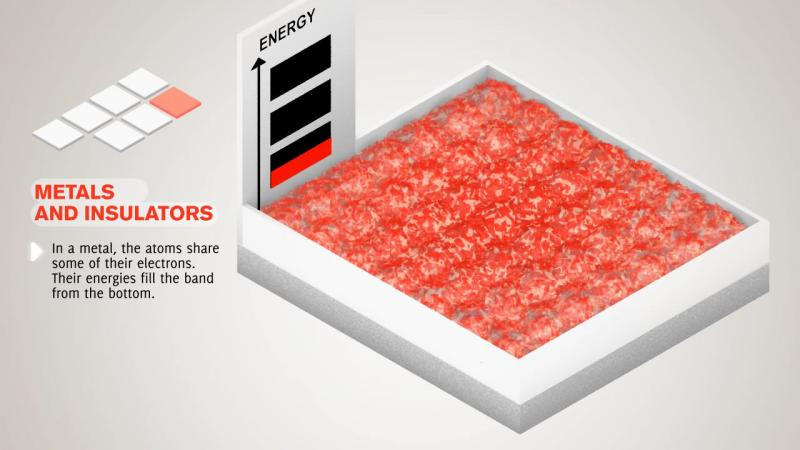
\includegraphics[width=.9\linewidth]{../figs/Metals_and_insulators_video.jpg}}
\end{frame}

\begin{frame}[label=sec-1-1-2]{Átomos aislados vs. Átomos en Sólido}
\begin{itemize}
\item Supongamos una red cristalina formada por átomos.

\item Los \alert{electrones de un átomo aislado} pueden existir \alert{únicamente en determinados estados de energía}.

\item A medida que disminuye la distancia interatómica comienza a observarse la \alert{interacción mutua entre los átomos} hasta formarse un sistema electrónico único.

\item Las \alert{fuerzas de repulsión y atracción} entre los átomos encontrarán su \alert{equilibrio} cuando los átomos estén separados por la \alert{distancia interatómica típica del cristal} que se trate.

\item La separación real entre átomos en el cristal será aquella para la cual la \alert{energía del sólido sea mínima}.
\end{itemize}
\end{frame}

\begin{frame}[label=sec-1-1-3]{Bandas de energía}
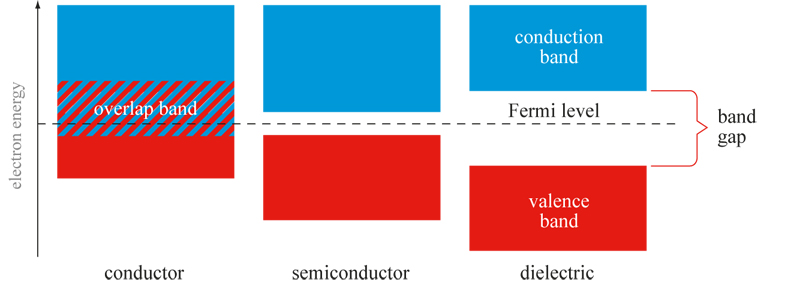
\includegraphics[width=.9\linewidth]{../figs/simplified_band_diagram.jpg}
\end{frame}

\begin{frame}[label=sec-1-1-4]{Bandas de energía}
\begin{itemize}
\item En un \alert{sólido} el número de átomos es tan elevado que los niveles de energía forman \alert{bandas continuas de energía}.

\item Los \alert{electrones} asociados a los átomos del sólido \alert{llenan estas bandas en orden ascendente}.

\item La banda de mayor energía completamente ocupada se denomina \alert{banda de valencia} (\emph{electrones ligados a átomos}). La siguiente banda, parcialmente ocupada o vacía, se denominada \alert{banda de conducción} (\emph{electrones desligados de átomos}).

\item Estas bandas pueden estar separadas por otra banda de energías que corresponde a \alert{estados no permitidos} (\alert{banda prohibida}), o \alert{pueden estar solapadas} permitiendo una transición fácil de una a otra.
\end{itemize}
\end{frame}

\begin{frame}[label=sec-1-1-5]{Bandas de energía}
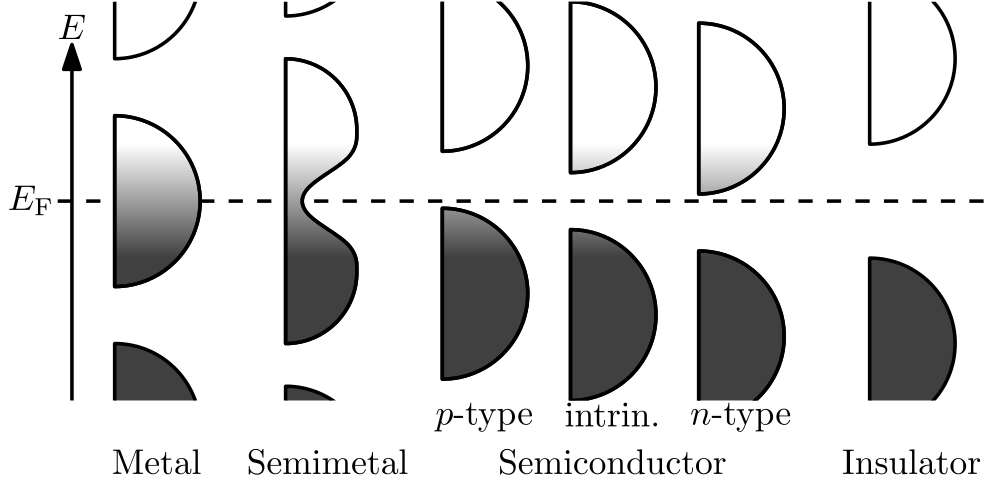
\includegraphics[width=.9\linewidth]{../figs/Band_filling_diagram.png}
\end{frame}

\begin{frame}[label=sec-1-1-6]{Conductores, aislantes y semiconductores}
Las \alert{propiedades eléctricas} del sólido dependen de esta \alert{posición relativa entre bandas}.

\begin{itemize}
\item En un \alert{conductor} la $E_{g}$ es muy baja y los electrones circulan fácilmente por la banda de conducción.

\item En un \alert{aislante} se necesita una cantidad de energía muy alta para que los electrones puedan acceder a la banda de conducción   ($E_{g}>\SI{5}{\electronvolt}$)

\item En un \alert{semiconductor} la $E_{g}$ es baja ($E_{g}<\SI{5}{\electronvolt}$): los electrones pueden \guillemotleft{}saltar\guillemotright{} a la banda de conducción con un aporte energético.

\begin{itemize}
\item Para el silicio $E_{g}=\SI{1.12}{\electronvolt}$.
\end{itemize}
\end{itemize}
\end{frame}

\subsection{Semiconductores}
\label{sec-1-2}

\begin{frame}[label=sec-1-2-1]{Rotura de Enlaces}
\begin{itemize}
\item Cuando se rompe un enlace, un electrón y un hueco quedan libres para moverse por el material (conducción intrínseca).

\item La \alert{densidad intrínseca de huecos y electrones es idéntica}. Esta densidad depende de la temperatura y de $E_{g}$.

\item Esta \alert{circulación es aleatoria}, sin una dirección predeterminada.
\end{itemize}
\end{frame}

\begin{frame}[label=sec-1-2-2]{Recombinación de un par electrón-hueco}
\begin{itemize}
\item Por tanto, se producen \alert{encuentros electrón-hueco} que restablecen un enlace con liberación de energia ($E_{g}$) en forma de calor.

\begin{itemize}
\item Las impurezas del cristal favorecen la recombinación.

\item El tiempo de vida de portadores mide cuánto tarda en producirse el proceso de recombinación.

\item La longitud de difusión de portadores mide la distancia media que puede recorrer un portador antes de ser recombinado.
\end{itemize}

\item Esta \alert{conducción intrínseca} \alert{no es aprovechable} en un circuito externo.

\item Para evitar la recombinación \alert{es preciso dirigir el movimiento} de electrones y huecos mediante un campo eléctrico.
\end{itemize}
\end{frame}

\subsection{Dopaje de semiconductores}
\label{sec-1-3}
\begin{frame}[label=sec-1-3-1]{Tipo n}
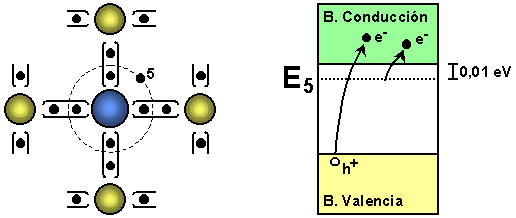
\includegraphics[width=.9\linewidth]{../figs/Semiconductor_tipo_n.png}
\end{frame}

\begin{frame}[label=sec-1-3-2]{Tipo n}
\begin{itemize}
\item El \alert{dopaje de semiconductores} consiste en introducir de forma
controlada impurezas en el cristal.

\item Los átomos de* Fósforo* tienen cinco electrones de valencia (uno más
que el silicio).

\item Al impurificar un cristal de Silicio con átomos de Fósforo, el quinto
electrón no queda bien integrado en la red.

\item La rotura de este enlace se produce con \alert{baja aportación energética}
   (menor que $E_{g}$).

\item El \alert{quinto electrón queda libre pero la carga positiva (ión $P^{+}$)
está ligada} a la red cristalina.

\item La \alert{densidad de electrones es superior a la de huecos}

\begin{itemize}
\item Semiconductor \alert{tipo n}.

\item El \alert{portador mayoritario} es el \alert{electrón}.
\end{itemize}
\end{itemize}
\end{frame}

\begin{frame}[label=sec-1-3-3]{Tipo p}
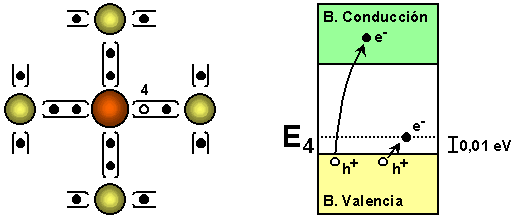
\includegraphics[width=.9\linewidth]{../figs/Semiconductor_tipo_p.png}
\end{frame}

\begin{frame}[label=sec-1-3-4]{Tipo p}
\begin{itemize}
\item Los átomos de \alert{Boro} tienen tres electrones de valencia (uno menos
que el silicio).

\item Al impurificar un cristal de Silicio con átomos de Boro, hay un
enlace sin cubrir (hueco).

\item La rotura de este enlace se produce con \alert{baja aportación energética}
   (menor que $E_{g}$).

\item El \alert{hueco queda libre} pero la \alert{carga negativa (ión $B^{-}$) está
ligada} a la red cristalina.

\item La \alert{densidad de huecos} es \alert{superior a la de electrones}

\begin{itemize}
\item Semiconductor \alert{tipo p}.

\item El \alert{portador mayoritario} es el \alert{hueco}.
\end{itemize}
\end{itemize}
\end{frame}

\subsection{Unión p-n}
\label{sec-1-4}


\begin{frame}[label=sec-1-4-1]{}
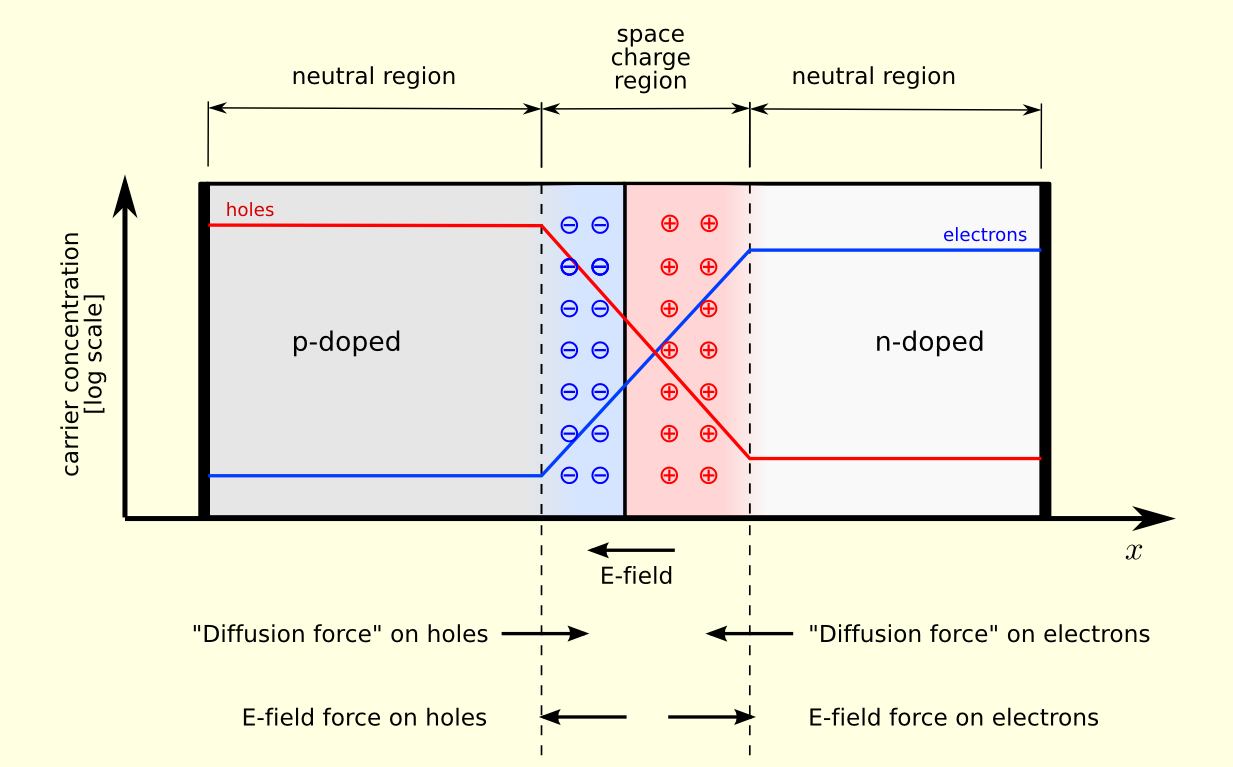
\includegraphics[width=.9\linewidth]{../figs/Pn-junction-equilibrium.png}
\end{frame}

\begin{frame}[label=sec-1-4-2]{Fundamentos}
\begin{itemize}
\item Al \alert{unir un semiconductor tipo p con otro tipo n, se produce un
desequilibrio}

\item \alert{Difusión de portadores mayoritarios}

\begin{itemize}
\item Hay un movimiento de huecos desde cristal p a cristal n, quedando
cargado negativamente.

\item Hay un movimiento de electrones desde cristal n a cristal p,
quedando cargado positivamente.
\end{itemize}

\item Este proceso de difusión también \alert{desequilibra} las densidades de
portadores en los cristales.

\item \alert{Proceso de arrastre}: Este desequilibrio \alert{crea un campo eléctrico}
(sentido del cristal n al cristal p) en contra del proceso de
difusión.

\item El \alert{equilibrio} se alcanza al \alert{compensarse los movimientos de
difusión y de arrastre}.
\end{itemize}
\end{frame}

\begin{frame}[label=sec-1-4-3]{Recombinación en una unión p-n}
\begin{itemize}
\item Los \alert{portadores minoritarios que atraviesan la unión se recombinan}:

\begin{itemize}
\item Electrones de cristal n con huecos en cristal p.

\item Huecos de cristal p con electrones en cristal n.
\end{itemize}

\item Esta recombinación deja \alert{iones cargados ligados a la red} (incapaces
de conducir)

\item Esta recombinación se produce en \alert{zonas cercanas a la unión} (zona de
carga de espacio)

\begin{itemize}
\item Despoblada de portadores

\item \alert{Los iones fijos generan un campo eléctrico de arrastre}.
\end{itemize}
\end{itemize}
\end{frame}

\begin{frame}[label=sec-1-4-4]{Polarización en directa}
\begin{itemize}
\item \alert{Para conseguir corriente es necesario romper el equilibrio alcanzado
y reducir el valor del potencial termodinámico}.

\item \alert{Diferencia de potencial} con lado p positivo respecto al lado n:
unión p-n está \alert{polarizada en directa}.

\item En estas condiciones \alert{se reduce la barrera de potencial} y, en
consecuencia el valor del campo eléctrico de la zona de unión.

\item La \alert{corriente de arrastre disminuye} y \alert{no puede compensar la
corriente de difusión}.

\item Aparecen dos corrientes en sentidos contrarios pero de partículas de
diferente signo: \alert{corriente total aprovechable.}

\item Convenio: la corriente entra por zona p y sale por zona n.
\end{itemize}
\end{frame}

\begin{frame}[label=sec-1-4-5]{Polarización en inversa}
\begin{itemize}
\item Si la diferencia de potencial aplicada consigue que la zona p esté a
menor tensión que la zona n, la unión queda \alert{polarizada en inversa}.

\item En estas condiciones \alert{la barrera de potencial en la unión queda
reforzada} y el paso de portadores de una a otra zona queda aún más
debilitado.

\item La \alert{corriente *que atraviesa la unión en polarización inversa es de
*muy bajo valor}.
\end{itemize}
\end{frame}

\subsection{Diodo}
\label{sec-1-5}

\begin{frame}[label=sec-1-5-1]{Definición}
\begin{itemize}
\item El dispositivo electrónico basado en una unión p-n se denomina diodo.

\item La zona p del diodo es el ánodo y la zona n es el cátodo.
\end{itemize}

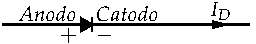
\includegraphics[width=.9\linewidth]{../figs/Diodo.pdf}
\end{frame}

\begin{frame}[label=sec-1-5-2]{Ecuación del Diodo}
$$I_{D}=I_{0}\cdot[\exp(\frac{V}{m\cdot V_{T}})-1]$$ donde $I_{0}$ es la
corriente de saturación en oscuridad del diodo, $V$ la tensión aplicada
al diodo y $m$ el factor de idealidad del diodo.

Para una temperatura ambiente de $\SI{300}{\kelvin}$,
$$V_{T}=\frac{\mathrm{k}T}{\mathrm{e}}=\SI{25.85}{\milli\volt}$$ donde
$\mathrm{k}$ es la constante de Boltzmann, $T$ la temperatura del diodo
(en grados Kelvin), y $\mathrm{e}$ es la carga del electrón.
\end{frame}

\begin{frame}[label=sec-1-5-3]{}
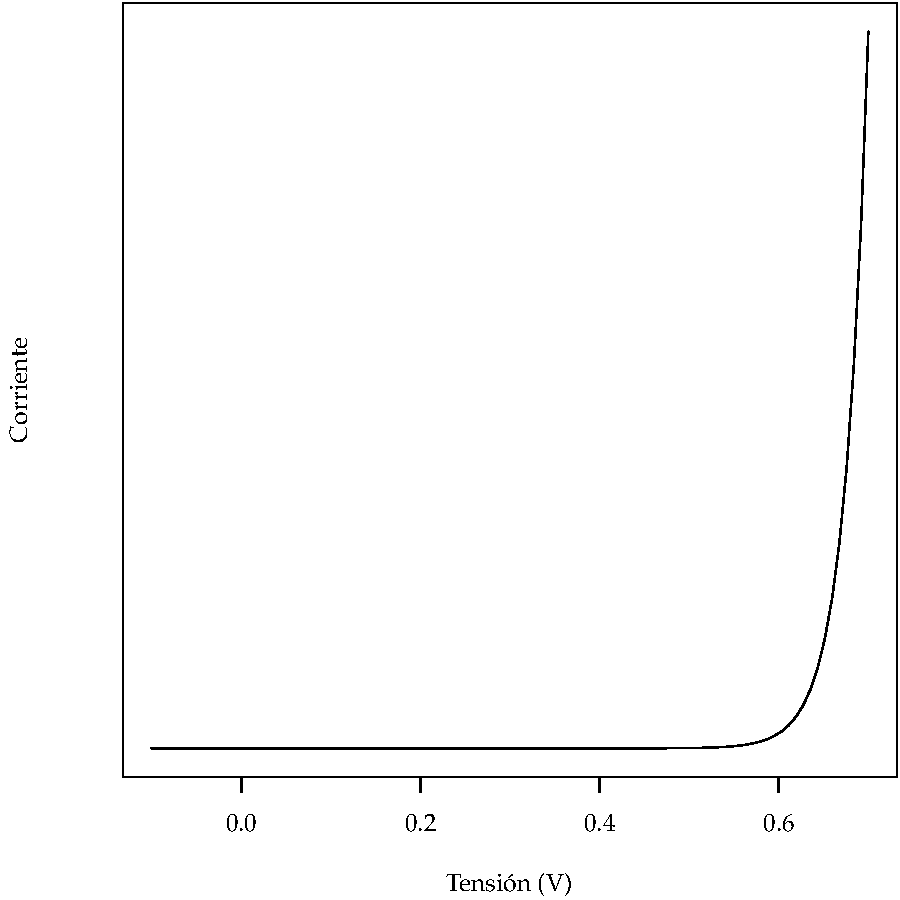
\includegraphics[width=.9\linewidth]{../figs/EcuacionDiodo.pdf}
\end{frame}

\section{Unión P-N iluminada}
\label{sec-2}

\begin{frame}[label=sec-2-0-1]{}
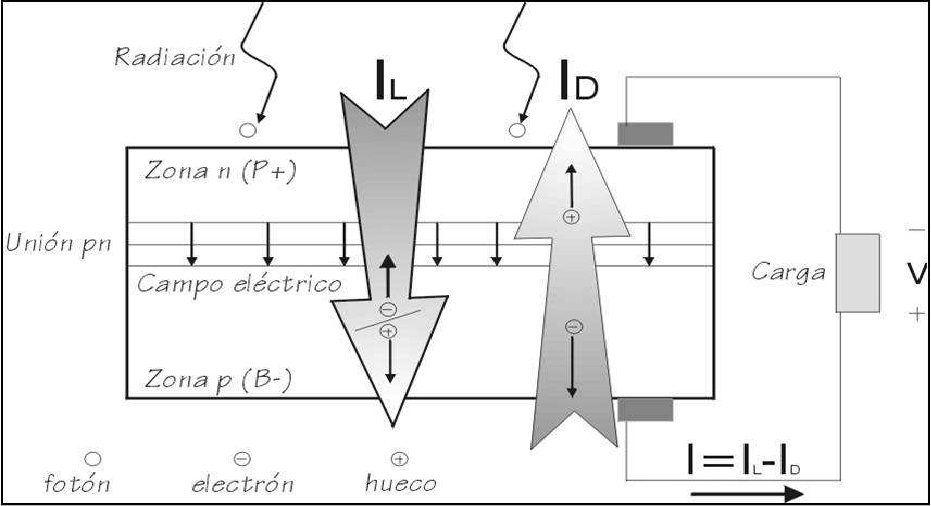
\includegraphics[width=.9\linewidth]{../figs/CelulaSolar.pdf}
\end{frame}

\begin{frame}[label=sec-2-0-2]{Efecto fotoeléctrico}
\begin{itemize}
\item Efecto fotoeléctrico: \alert{los electrones se desplazan a la banda de
conducción por el aporte energético de fotones}
($E_{f}=\frac{h\cdot c}{\lambda}$).

\item Al \alert{iluminar una unión p-n}, el \alert{campo eléctrico} de la unión conduce
los portadores y \alert{dificulta la recombinación}.

\item La \alert{fotocorriente} es ahora \alert{aprovechable} por un circuito externo
(\emph{corriente de iluminación, corriente de generación})

\item La presencia de \alert{tensión en los terminales} de la unión (por ejemplo,
caída de tensión en una resistencia alimentada por la fotocorriente)*
favorece la recombinación* (\emph{corriente de oscuridad o corriente de
diodo}).
\end{itemize}

$$I=I_{L}-I_{0}\cdot[\exp(\frac{V}{m\cdot V_{T}})-1]$$
\end{frame}

\begin{frame}[label=sec-2-0-3]{Absorción de luz y generación de portadores}
\begin{itemize}
\item Si el \alert{fotón es poco energético} ($E_{f}<E_{g}$) \alert{no interactúa con
el semiconductor} (como si fuese transparente)

\begin{itemize}
\item Fotones en el espectro visible ($400\, nm<\lambda<700\, nm$) y
ultravioleta ($\lambda<400\, nm$) rompen enlaces.

\item Si $\lambda>1100\, nm$ (infrarrojo) el fotón no interactúa.
\end{itemize}

\item Los* fotones más energéticos \alert{(baja longitud de onda) son *absorbidos
en la superficie}.

\item Los \alert{fotones menos energéticos} (alta longitud de onda) penetran en
el interior hasta \alert{romper un enlace}.
\end{itemize}
\end{frame}

\begin{frame}[label=sec-2-0-4]{Absorción de luz y generación de portadores}
\begin{itemize}
\item Los fotones con $E_{f}<E_{g}$ atraviesan el cristal sin ser
absorbidos: \alert{pérdidas de no-absorción}

\item Fotones con $E_{f}>E_{g}$:

\begin{itemize}
\item Debido a anchura del semiconductor y coeficiente de absorción del
material parte no son absorbidos: \alert{pérdidas de transmisión}

\item Debido a diferencia de índices de refracción: \alert{pérdidas de
reflexión}

\item Parte de los portadores generadores se recombinan dentro del
dispositivo: \alert{pérdidas por recombinación}
\end{itemize}
\end{itemize}

$$I_{L}<e\cdot A\cdot\intop_{E_{G}}^{\infty}S(E)\mathrm{d}E$$
\end{frame}

\section{Funcionamiento de una célula solar}
\label{sec-3}

\subsection{Curva IV y Puntos Característicos}
\label{sec-3-1}
\begin{frame}[label=sec-3-1-1]{Característica I-V de iluminación}
$$I=I_{L}-I_{D}$$

$$I_{D}=I_{0}\cdot\left[\exp\left(\frac{e\cdot V}{m\cdot k\cdot
      T_{c}}\right)-1\right]$$

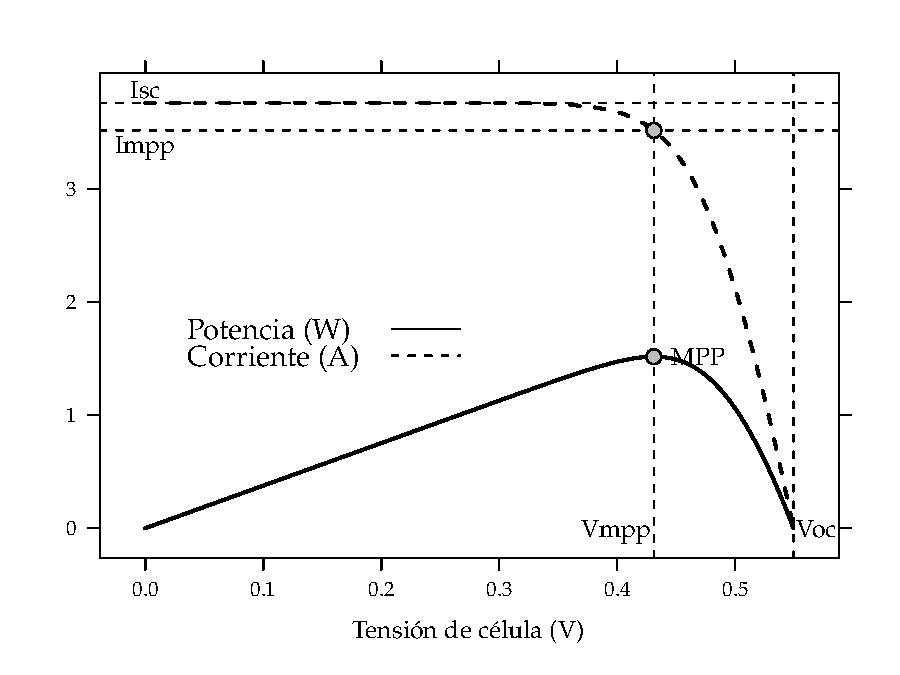
\includegraphics[width=.9\linewidth]{../figs/CurvaIV_Ta20_G800.pdf}
\end{frame}

\begin{frame}[label=sec-3-1-2]{Isc y Voc}
\begin{itemize}
\item Corriente de Cortocircuito
\end{itemize}

$$I_{sc}=I(V=0)\Rightarrow I_{D}=0\Rightarrow I=I_{L}$$

\begin{itemize}
\item Tensión de Circuito Abierto
\end{itemize}

$$V_{oc}=V(I=0)\Rightarrow I_{L}=I_{D}\Rightarrow
V_{oc}=m\cdot\frac{k\cdot
  T_{c}}{e}\cdot\ln\left(\frac{I_{L}}{I_{0}}+1\right)$$

\begin{itemize}
\item Ecuación general
\end{itemize}

$$I=I_{sc}\cdot\left[1-\exp\left(\frac{e\cdot(V_{oc}-V)}{m\cdot k\cdot
      T_{c}}\right)\right]$$
\end{frame}

\begin{frame}[label=sec-3-1-3]{Punto de máxima potencia}
$$\frac{dP}{dV}=0$$

$$\frac{d(I\cdot
  V)}{dV}=V\cdot\frac{dI(V)}{dV}+I\cdot\frac{dV}{dV}\Rightarrow
dP=V\cdot dI+I\cdot dV$$
\end{frame}



\begin{frame}[label=sec-3-1-4]{Punto de máxima potencia}
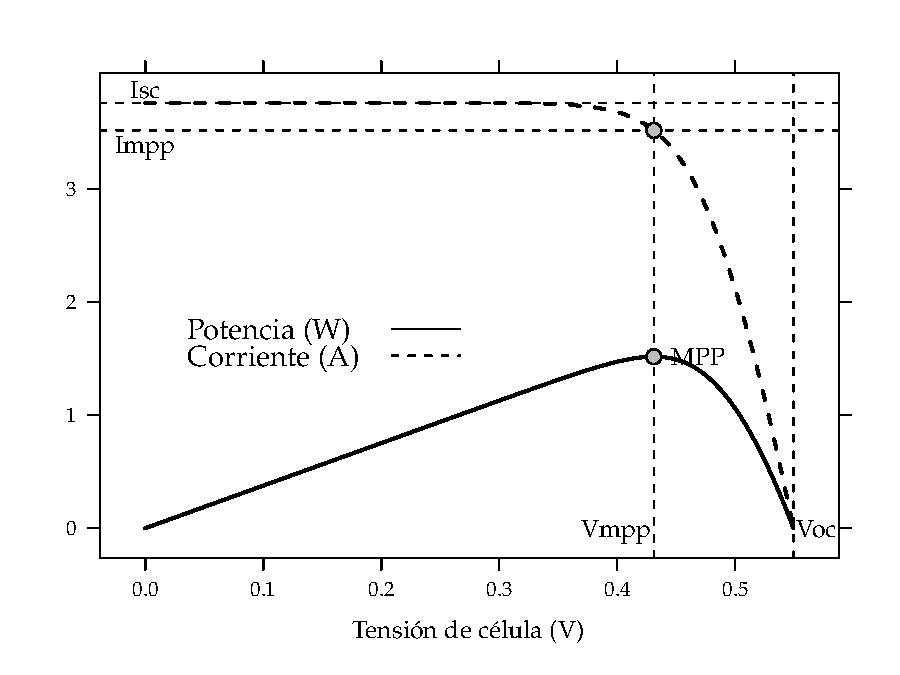
\includegraphics[width=.9\linewidth]{../figs/CurvaIV_Ta20_G800.pdf}

$V=V_{mpp}:\,\frac{dI}{dV}=-\frac{I}{V}$

$0<V<V_{mpp}$:  $\frac{dP}{dV}>0\Rightarrow\frac{dI}{dV}>-\frac{I}{V}$

$V_{mpp}<V<V_{oc}$: 
$\frac{dP}{dV}<0\Rightarrow\frac{dI}{dV}<-\frac{I}{V}$
\end{frame}

\begin{frame}[label=sec-3-1-5]{Factor de forma y Eficiencia}
\begin{itemize}
\item Factor de Forma
\end{itemize}
$$FF=\frac{I_{mpp}\cdot V_{mpp}}{I_{sc}\cdot V_{oc}}$$

$$P_{mpp}=FF\cdot I_{sc}\cdot V_{oc}$$

\begin{itemize}
\item Eficiencia
\end{itemize}

$$\eta=\frac{I_{mpp}\cdot V_{mpp}}{P_{L}}$$
\end{frame}

\begin{frame}[label=sec-3-1-6]{Eficiencia de células}
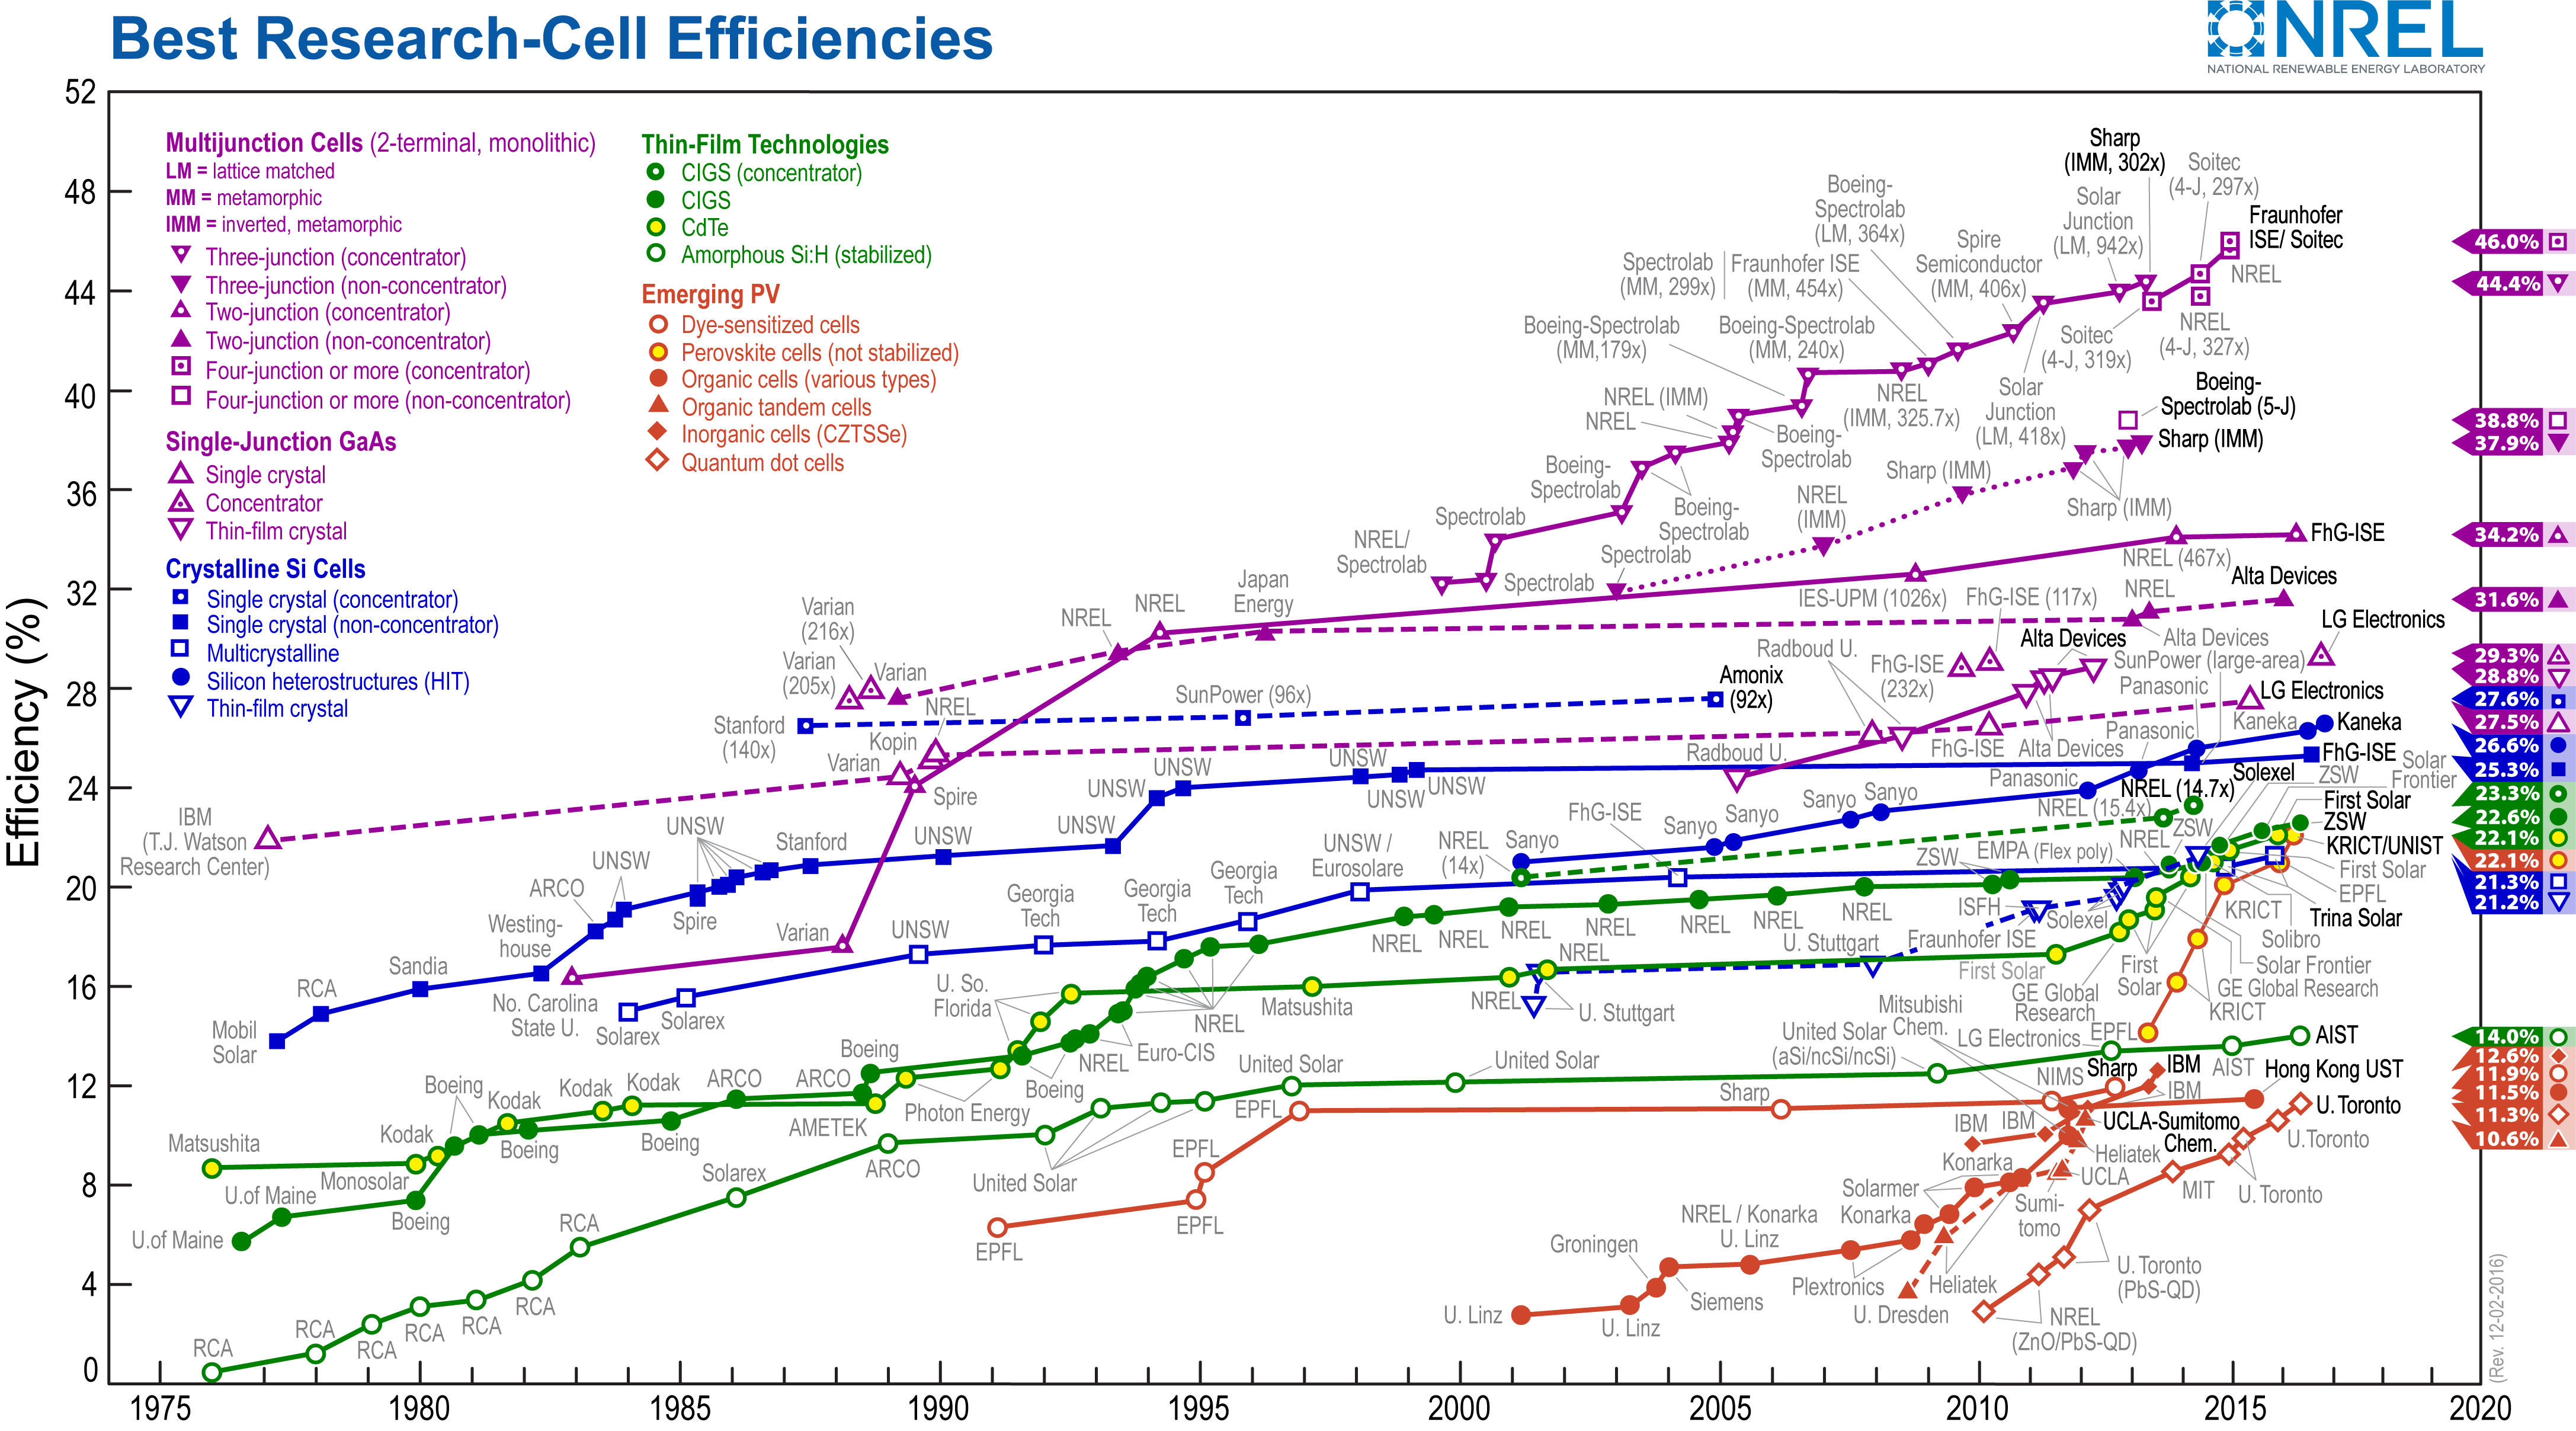
\includegraphics[width=1\textwidth]{../figs/efficiency_chart_nrel.jpg}

\url{http://www.nrel.gov/ncpv/}
\end{frame}

\subsection{Circuito equivalente de la célula}
\label{sec-3-2}

\begin{frame}[label=sec-3-2-1]{Circuito equivalente}
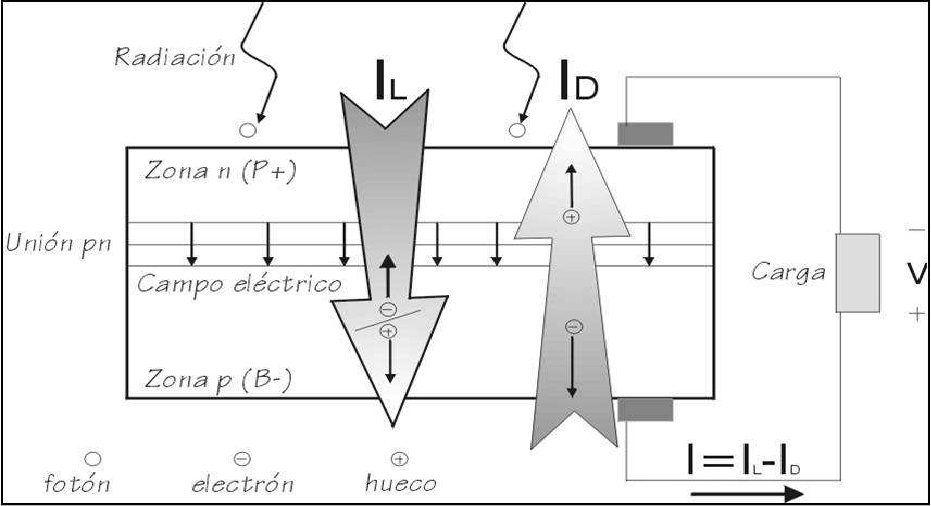
\includegraphics[width=.9\linewidth]{../figs/CelulaSolar.pdf}

$$I=I_{L}-I_{0}\cdot[\exp(\frac{V+I\cdot R_{s}}{m\cdot
  V_{T}})-1]-\frac{V+I\cdot R_{s}}{R_{p}}$$

\begin{itemize}
\item Ecuación simplificada
\end{itemize}

$$I=I_{sc}[1-\exp(\frac{V-V_{oc}+I\cdot R_{s}}{m\cdot V_{t}})]$$
\end{frame}

\begin{frame}[label=sec-3-2-2]{Resistencia Serie}
\begin{itemize}
\item Resistencia de contactos metálicos con el semiconductor

\item Resistencia de capas semiconductoras

\item Resistencia de malla de metalización
\end{itemize}

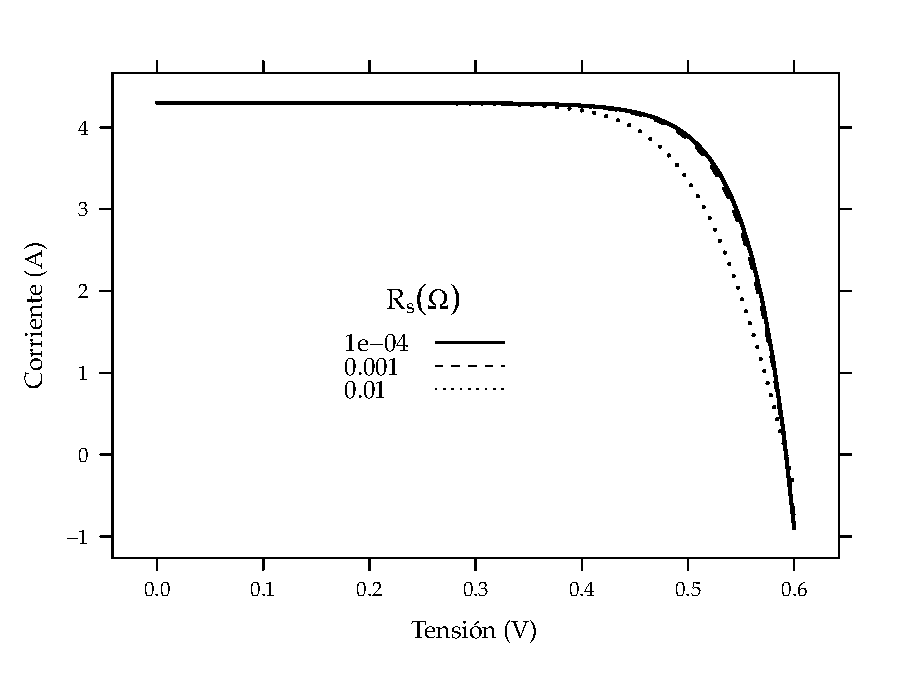
\includegraphics[width=.9\linewidth]{../figs/InfluenciaRs_IV.pdf}
\end{frame}

\begin{frame}[label=sec-3-2-3]{Resistencia Serie}
\begin{itemize}
\item Resistencia de contactos metálicos con el semiconductor

\item Resistencia de capas semiconductoras

\item Resistencia de malla de metalización
\end{itemize}

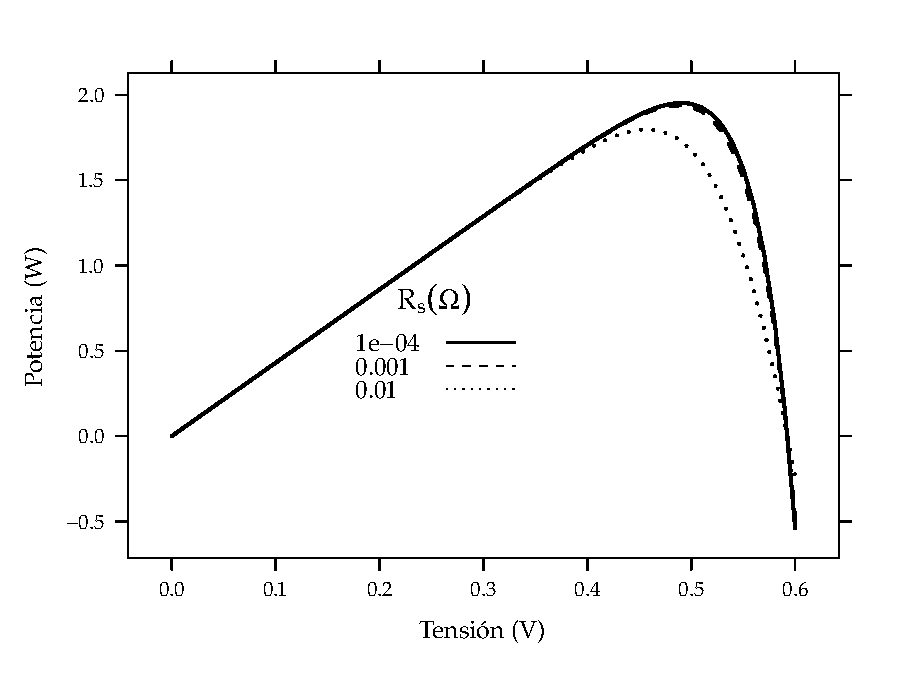
\includegraphics[width=.9\linewidth]{../figs/InfluenciaRs_Potencia.pdf}
\end{frame}

\begin{frame}[label=sec-3-2-4]{Resistencia paralelo}
\begin{itemize}
\item Fugas de corriente en bordes de célula

\item Cortocircuitos metálicos

\item Caminos de difusión en fronteras de grano
\end{itemize}

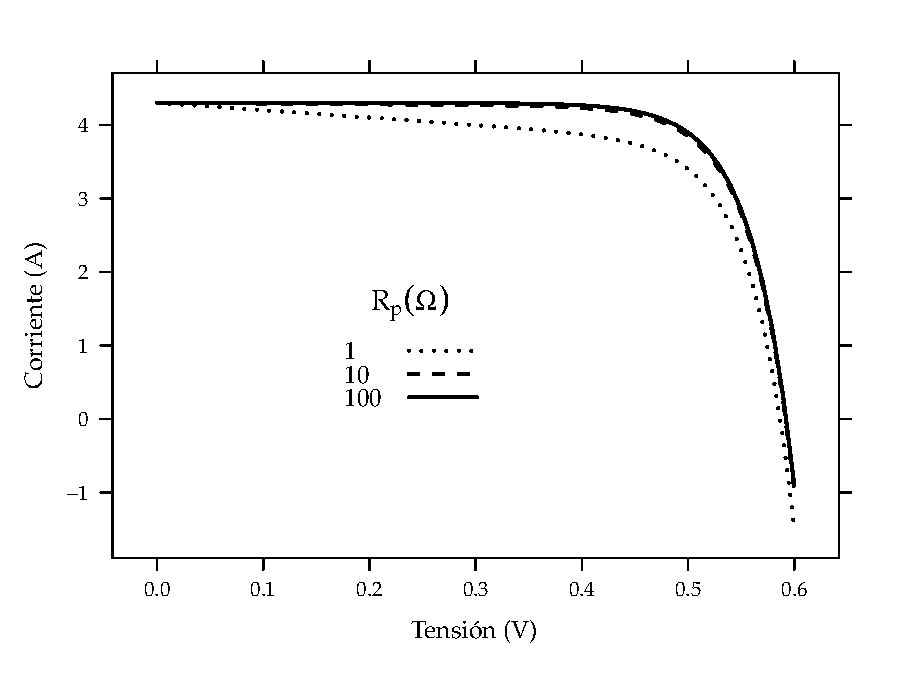
\includegraphics[width=.9\linewidth]{../figs/InfluenciaRsh_IV.pdf}
\end{frame}

\begin{frame}[label=sec-3-2-5]{Resistencia paralelo}
\begin{itemize}
\item Fugas de corriente en bordes de célula

\item Cortocircuitos metálicos

\item Caminos de difusión en fronteras de grano
\end{itemize}

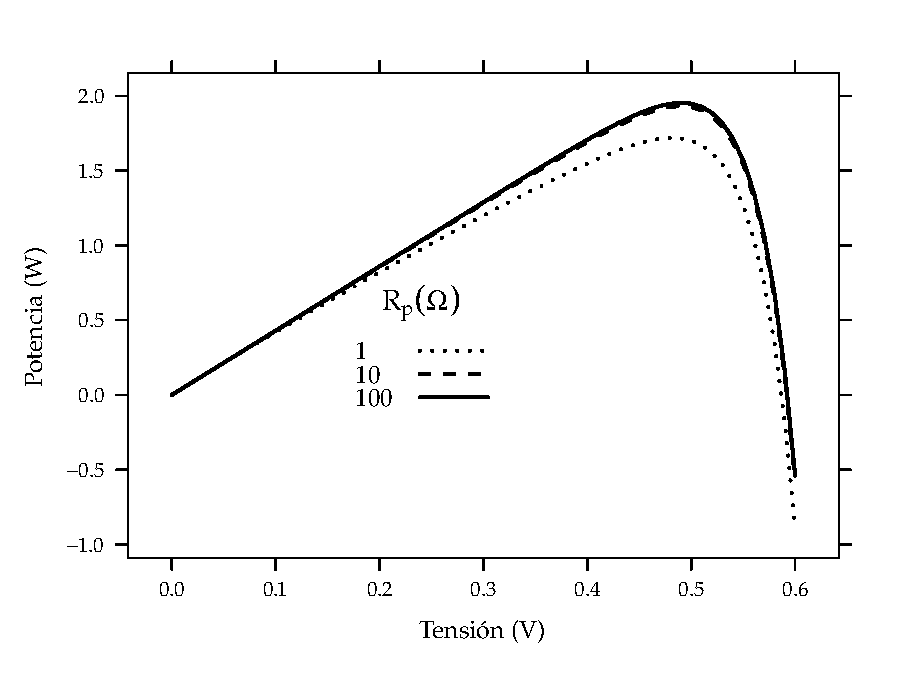
\includegraphics[width=.9\linewidth]{../figs/InfluenciaRsh_Potencia.pdf}
\end{frame}

\subsection{Influencia de Temperatura y Radiación}
\label{sec-3-3}

\begin{frame}[label=sec-3-3-1]{Radiación}
\begin{itemize}
\item Fotocorriente proporcional a intensidad de radiación

\item Relación logarítmica con tensión de circuito abierto:
$V_{oc}=V_{oc1}+\frac{mkT}{e}\cdot\ln(X)$

\item El factor de forma aumenta ligeramente

\item La eficiencia crece de forma logarítmica hasta determinado nivel.
\end{itemize}
\end{frame}

\begin{frame}[label=sec-3-3-2]{Influencia de la Radiación}
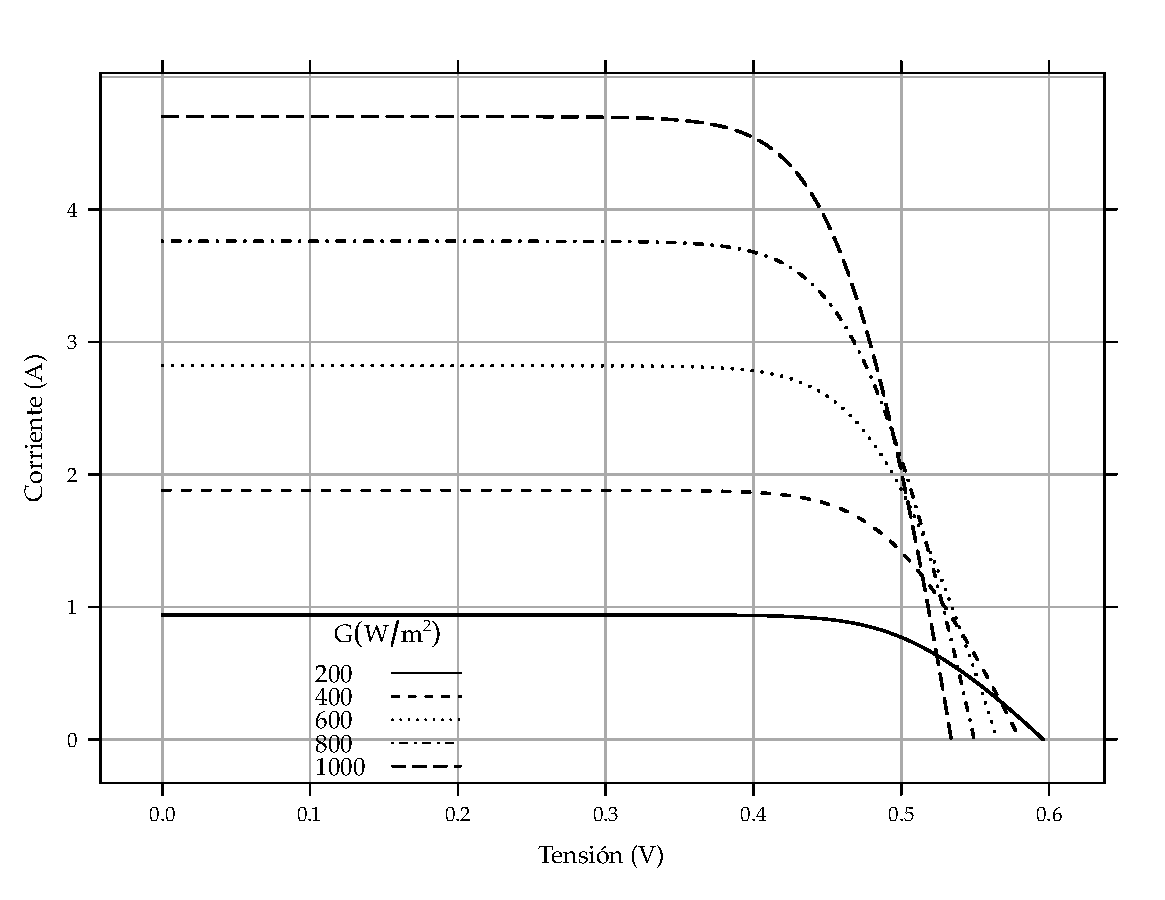
\includegraphics[width=.9\linewidth]{../figs/CurvaIV_Ta20.pdf}
\end{frame}

\begin{frame}[label=sec-3-3-3]{Temperatura}
\begin{itemize}
\item Se estrecha el salto entre banda de valencia y conducción: aumenta
\emph{ligeramente} la fotocorriente

\item Disminuye la tensión de circuito
abierto:$dV_{oc}/dT_{c}=\SI{-2.3}{\milli\volt\per\celsius}$

\item Disminuye el factor de forma y la eficiencia:
$d\eta/dT_{c}=\SI{-0.4}{\percent\per\celsius}$
\end{itemize}
\end{frame}

\begin{frame}[label=sec-3-3-4]{Influencia de Temperatura}
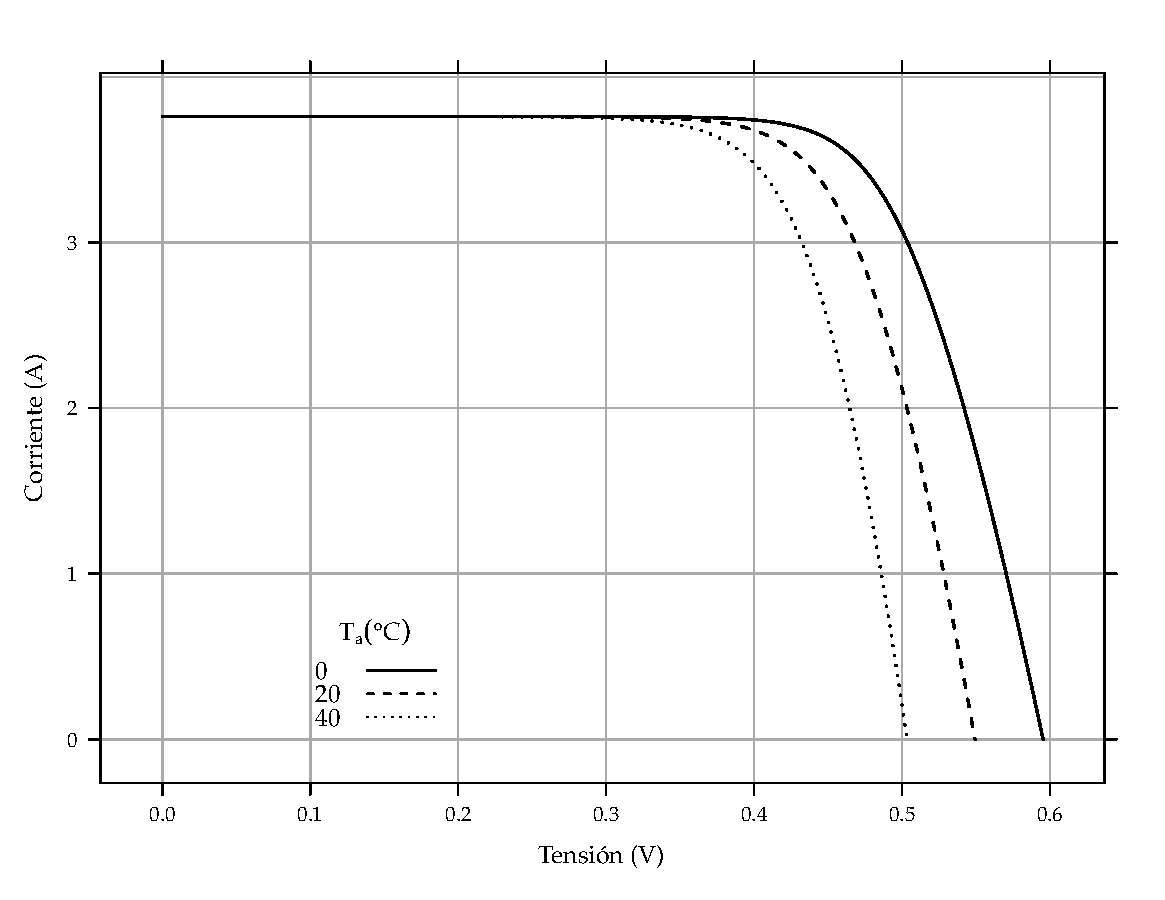
\includegraphics[width=.9\linewidth]{../figs/CurvaIV_G800.pdf}
\end{frame}

\begin{frame}[label=sec-3-3-5]{Condiciones Estándar de Medida}
\begin{itemize}
\item Irradiancia: $G^{*}=\SI{1000}{\watt\per\meter\squared}$ con
incidencia normal.

\item Temperatura de célula: $T_{c}^{*}=\SI{25}{\celsius}$.

\item Masa de aire: $AM=1.5$
\end{itemize}

$$P_{mpp}^{*}=I_{mpp}^{*}\cdot V_{mpp}^{*}$$

$$\eta^{*}=\frac{I_{mpp}^{*}\cdot V_{mpp}^{*}}{A\cdot G^{*}}$$
\end{frame}

\subsection{Cálculo del MPP}
\label{sec-3-4}

\begin{frame}[label=sec-3-4-1]{Método de J.M. Ruiz}
\begin{itemize}
\item Normalización
\end{itemize}

$$\begin{aligned}
  v & = & \frac{V}{V_{oc}}\\
  i & = & \frac{I}{I_{sc}}\end{aligned}$$

\begin{itemize}
\item MPP
\end{itemize}

$$\begin{aligned}
  v_{mpp} & = & \frac{V_{mpp}}{V_{oc}}\\
  i_{mpp} & = & \frac{I_{mpp}}{I_{sc}}\\
  p_{mpp} & = & FF\end{aligned}$$
\end{frame}

\begin{frame}[label=sec-3-4-2]{Método de J.M. Ruiz}
\begin{itemize}
\item Resistencia Serie y FF
\end{itemize}

$$\begin{aligned}
  r_{s} & = & \frac{R_{s}}{(V_{oc}/I_{sc})}\\
  ff & = & v_{mpp}\cdot i_{mpp}=FF\end{aligned}$$

\begin{itemize}
\item Tensión térmica
\end{itemize}

$$\begin{aligned}
  k_{oc} & = & \frac{V_{oc}}{V_{t}}\end{aligned}$$
\end{frame}

\begin{frame}[label=sec-3-4-3]{Método de J.M. Ruiz}
\begin{itemize}
\item Aproximación para MPP
\end{itemize}

$$\begin{aligned}
  i_{mpp} & = & 1-\frac{D_{M}}{k_{oc}}\\
  v_{mpp} & = & 1-\frac{\ln(k_{oc}/D_{M})}{k_{oc}}-r_{s}\cdot i_{mpp}\end{aligned}$$

$$\begin{aligned}
  D_{M} & = & D_{M0}+2\cdot r_{s}\cdot D_{M0}^{2}\\
  D_{M0} & = & \frac{k_{oc}-1}{k_{oc}-\ln k_{oc}}\end{aligned}$$
\end{frame}

\begin{frame}[label=sec-3-4-4]{Método de J.M. Ruiz}
\begin{itemize}
\item Itinerario

\begin{itemize}
\item Obtener los valores de $I_{sc}$ y $V_{oc}$ en las condiciones de
temperatura y radiación deseadas

\item Obtener resistencia serie (supondremos $R_{s}=R_{s}^{*}$)
$$R_{s}^{*}=\frac{V_{oc}^{*}-V_{mpp}^{*}+m\cdot
            V_{t}\cdot\ln(1-\frac{I_{mpp}^{*}}{I_{sc}^{*}})}{I_{mpp}^{*}}$$
donde se debe emplear el valor de $V_{t}$ para
$T_{c}=\SI{25}{\celsius}$.

\item Calcular $r_{s}$ y $k_{oc}$, y con ellos $D_{M0}$ y $D_{M}$.

\item Calcular $i_{mpp}$ y a continuación $v_{mpp}$.

\item Deshacer la normalización para obtener $I_{mpp}$ y $V_{mpp}$.
\end{itemize}
\end{itemize}
\end{frame}

\begin{frame}[label=sec-3-4-5]{Simplificado: Factor de Forma Constante}
$$FF=FF^{*}$$

$$\begin{aligned}
  \frac{I_{mpp}}{I_{sc}} & = & \frac{I_{mpp}^{*}}{I_{sc}^{*}}\\
  \frac{V_{mpp}}{V_{oc}} & = & \frac{V_{mpp}^{*}}{V_{oc}^{*}}\end{aligned}$$
\end{frame}

\begin{frame}[label=sec-3-4-6]{Ejercicio de Cálculo}
De una célula de $\SI{100}{\centi\meter\squared}$ y $I_{sc}^{*}=3\, A$, $I_{mpp}^{*}=2.7\, A$ , $V_{oc}^{*}=0.6\, V$,
$V_{mpp}^{*}=0.48\, V$, calcular suponiendo factor de forma constante:

\begin{itemize}
\item $P_{mpp}^{*}$, $FF^{*}$, $\eta^{*}$

\item $I_{mpp}$, $V_{mpp}$ cuando $T_{c}=60\celsius$ y $G=800\, W/m^{2}$.
\end{itemize}
\end{frame}

\section{Fabricación}
\label{sec-4}

\begin{frame}[label=sec-4-0-1]{Purificación de silicio}
\begin{itemize}
\item El silicio puede extraerse de la cuarzita obteniendo Silicio de grado
metalúrgico (98\% pureza).

\item Para la industria de la electrónica se necesita silicio de grado
electronico (nivel de impureza por debajo de $10^{-10}$, 9 nueves).

\item Para las células solares puede utilizarse silicio de grado solar
(nivel de impureza algo mayor).

\item Al mezclar silicio con acido clorhídrico se produce triclorosilano,
que es destilado para eliminar impurezas.

\item Al unir silano de cloro con hidrógeno se obtiene de vuelta silicio,
válido para células policristalinas (varios cristales en cada célula)
\end{itemize}
\end{frame}

\begin{frame}[label=sec-4-0-2]{Formación de obleas}
\begin{itemize}
\item Para obtener mayor pureza se emplea el silicio monocristalino (un
sólo cristal) obtenido mediante el proceso de Czochralski o similar
(se utiliza una semilla de cristal para crecer silicio a muy alta
temperatura).

\item El lingote resultante debe ser cortado en obleas de $200-500\,\mu m$.

\item Las obleas son sometidas a limpieza para eliminar impurezas por el
cortado.

\item A continuación, son dopadas con Fósforo y Boro para crear la unión
p-n.

\item Se limpian los bordes para evitar la formación de cortocircuitos
entre las zonas p y n.
\end{itemize}
\end{frame}

\begin{frame}[label=sec-4-0-3]{Formación de células}
\begin{itemize}
\item Se añaden los contactos posterior (alto recubrimiento) y anterior
(optimización para obtener baja $R_{s}$ y poco sombreado) empleando
aleaciones de plata y aluminio.

\item Para reducir las pérdidas por reflexión se añade una capa
antireflectante con (p.ej) óxido de Titanio (color azulado).

\item Si es posible, se textura la superficie (creación de mini pirámides).
\end{itemize}
\end{frame}
% Emacs 24.4.1 (Org mode 8.2.7c)
\end{document}